\documentclass[acmsmall]{acmart}
\AtBeginDocument{%
  \providecommand\BibTeX{{%
    \normalfont B\kern-0.5em{\scshape i\kern-0.25em b}\kern-0.8em\TeX}}}

% \graphicspath{images}
%% \citestyle{acmauthoryear}
\usepackage{float}
\usepackage{prftree}

\begin{document}
\title{A brief survey on Type Theory}

\author{Yee-Jian Tan}
\email{yeejian.tan@u.nus.edu}
\orcid{0000000257259633}
\affiliation{
  \institution{National University of Singapore}
  \country{Singapore}
  \postcode{138595}
}

\begin{abstract}
  This is a survey article on Martin-Lof's Type Theory.
\end{abstract}

\begin{CCSXML}
<ccs2012>
   <concept>
       <concept_id>10003752.10003790.10011740</concept_id>
       <concept_desc>Theory of computation~Type theory</concept_desc>
       <concept_significance>500</concept_significance>
       </concept>
   <concept>
       <concept_id>10003752.10003790.10003796</concept_id>
       <concept_desc>Theory of computation~Constructive mathematics</concept_desc>
       <concept_significance>300</concept_significance>
       </concept>
   <concept>
       <concept_id>10003752.10003790.10003800</concept_id>
       <concept_desc>Theory of computation~Higher order logic</concept_desc>
       <concept_significance>300</concept_significance>
       </concept>
 </ccs2012>
\end{CCSXML}

\ccsdesc[500]{Theory of computation~Type theory}
\ccsdesc[300]{Theory of computation~Constructive mathematics}
\ccsdesc[300]{Theory of computation~Higher order logic}

\keywords{Intuitionistic Type Theory, Calculus of Inductive Constructions,
  Martin-Lof Type Theory}

\maketitle

\section{Introduction}
\subsection{Background}
Type Theory lies in the intersection of logic and computer science. It was first
introduced by Russell in 1903 as a solution to the famous Russell's Paradox in
set theory~\cite{coquand2019type}, that the set of all sets (also the class of
all classes) cannot exist. Type theory solves this problem by establishing a
hierachy of objects, predicates, predicates of predicates etc.\ in a hierachy
now known as the extensional hierachy. These schema is proved to solve the
fundamental paradox lying at the roots of set theory raised by himself. At this
point, type theory was still just a mathematical theory about logic.

The connection between the Type Theory and computer science is made possible
after Alonzo Church invented the Lambda Calculus as an investigation into the
models of computation in the 1930s~\cite{church1932postulates}. The Lambda
Calculus (LC) is a small system of computation which consists only of functions
and their applications. Since lambda calculus is untyped by design, the
investigation of assigning types to lambda calculus terms and their rules led to
what was known as Type Theory in Computer Science now.

In this paper, we will focus more on the systems that derived from the attempts
to type different variations of lambda calculus, from the Simply Typed Lambda
Calculus (STLC) to the most recent Homotopy Type Theory (HoTT). This survey
paper will assume basic knowledge about propositional and predicate logic, as
well as some familiarity with programming types, or even better, abstract data
types such as pairs, functions and functionals (higher-order functions).
Although we will go through the fundamentals of lambda calculus briefly,
prerequisite knowledge about lambda calculus is not required but recommended.

\subsection{Overview}

Section~\ref{sec:tt} will give a brief introduction on lambda calculus and type
systems, before looking at their combination: typed lambda calculus.
Furthermore, we will establish the correspondence between logic and type theory.
After this section, all analysis will look at the two sides of typed lambda
calculus, type theory as a basis for functional programming languages, and type
theory as a logical system due to its correspondence to logic.

Section~\ref{sec:history} will look at the different systems of typed Lambda Calculus
chronologically, and discuss their roles in these 2 aspects: as functional
programming language and as a logic system.

Section~\ref{sec:application} will look at the current proof assistants and programming
languages, as well as dicussing the type theory systems behind the hood. This
provides an insight into how type theory is used in practice.

In the last section, Section~\ref{sec:future} we will look at current research
trends and what progress has been made, as well as what are the possible
directions for future research.



\section{Introduction to Type Theory}\label{sec:tt}

\subsection{Lambda Calculus}
The Lambda Calculus is, in modern terms, a system consists of purely
``functions'' and ``function calls'', on a \textbf{untyped} system without any data
structures. The specification for objects in Lambda Calculus, called
\emph{items}, is extremely short:
\begin{enumerate}
  \item Every variable (usually $x, y, z, t, \ldots$) is a Lambda Calculus term
        (called \emph{term} from here on).
  \item If $M$ is a term, then the abstraction (function) $\lambda x. M$ is a term.
  \item If $M, N$ are terms, then $M N$ (application) is a term.
\end{enumerate}

The syntax can be written succintly as $e ::= x\ |\ \lambda x.e\ |\ e\ e$, each branch
corresponding to the written rule above. The simple syntax and the sole idea of
\textbf{abstraction} provided a way to \textbf{create terms based on terms}, a
feature which be extended and discussed in Section~\ref{sec:lambdacube}.

\subsection{Simply Typed Lambda Calculus (SDLC)}
The \emph{SDLC} was invented in 1940 by Alonzo Church, not long after he
formulated the (untyped) lambda calculus (\cite{church1940formulation}). The
typing rule fairly simple: the types start by having a base types $B$, then
types are either in $B$ or is an ``arrow type'':
\begin{align*}
  \tau ::=  \tau\to \tau\ |\ T \quad \text{where }T\in B.
\end{align*}

\subsection{Types in Computer Programming}
In computer programming, the term ``types'' usually refer to the categories of
different data structures that programs compute, such as real numbers,
floating-point numbers (finite-precision real numbers), integers and more. These
are examples of concrete types in programming.

On the other hand, types without a contrete representation is called
\textbf{abstract types.} Since the lambda calculus does not come with constructs
such as numbers, characters or strings, the typing of it is inevitably abstract.
This led to the investigation of typing on lambda calculus, of which the most
intuitive form is known as ``Simply Typed Lambda Calculus'' (SDLC).

It is important to note that abstract programming types have a similar
formulation from the type in Type Theory or logic, and the implementation of
such mathematical types differe in programming languages and proof assistants.

\subsection{Curry-Howard correspondence}
There are 3 main findings in the Curry-Howard Correspondence
(\cite{howard1980formulae},\cite{Curry584}), the most relevant to this paper being:
\[\text{Natural Deduction corresponds to Typed Lambda Calculus.}\]

The correspondence requires an isomorphism, ie., it is proven that
\begin{enumerate}
  \item Every statement in the logical system can be represented as a term in
        typed lambda calculus.
  \item Every valid typed lambda calculus term corresponds to a statement in the
        natural deduction logical system.
\end{enumerate}

It is paramount to get an intuivite idea of this correspondence because it forms
the backbone of the rest of the paper. We outline it on Table~\ref{tab:chcorr}:

\begin{table}[H]
  \caption{Curry-Howard Correspondence}\label{tab:chcorr}
  \begin{tabular}{ll}
    \toprule
    Natural Deduction& Lambda Calculus\\
    \midrule
    lambda calculus terms & proofs\\
    types & propositions\\
    $p$ has type $P$ & $p$ is a proof of $P$\\
    $p\implies q$& $(\lambda x.y) : P\to Q$\\
  \bottomrule
\end{tabular}
\end{table}

This idea of ``proposition as types, proofs as programs'' sees extensions with
the invention of different extensions of the \emph{Simply Typed Lambda Calulus},
with its limited feature, corresponds to \emph{propositional logic}.

\subsection{The Lambda Cube}\label{sec:lambdacube}

Typed Lambda Calculus has two main constructs --- terms (or objects) and types.
Untyped Lambda Calculus allows terms to depend on terms (via the abstraction
rule), hence typed lambda calculus as well. A natural question to ask is: can we
generate terms/types using other terms/types, or conversely, have term/types
depend on other terms/types?

All the $2\times2$ possibilities are well-investigated by different type systems. We
list their formal names below:
\begin{table}[H]
  \caption{Definition of Typed Lamda Calculus features}\label{tab:term-type}
\begin{tabular}{llll}
  \toprule
  Generate & Using & Known as & Example\\
  \midrule
  Terms & Terms & \textbf{Abstraction}    & Identity Function: $\lambda x.x$\\
  Terms & Types & \textbf{Polymorphism}   & Polymorphic Identity Function: $\Lambda \alpha.\lambda x.x$\\
  Types & Terms & \textbf{Dependent Types}& Class of types indexed by $A$: $\prod_{x:A}B(x)$\\
  Types & Types & \textbf{Type Constructors} & \verb|TREE|$:=\lambda A:*.\prod B.(A\to B)\to(B\to B\to B)\to B$\\
  \bottomrule
\end{tabular}
\end{table}

We know that \emph{Simply Typed Lambda Calculus} only has \textbf{abstraction}
since it is just contains naively typed lambda calculus and nothing more. On top
of \emph{STLC}, a Type Theory can have any combination of other 3 features,
creating $2^{3}=8$ possibilities.

The Lambda Cube is a visual representation of the inclusion of these 4 features
in different type theories, introduced by Henk Barendregt\cite{barendregt_1991}
in 1991. It has three axes:
\begin{itemize}
  \item $x$-axis$(\rightarrow)$ represents \textbf{dependent types}, allowing
        \textbf{types to depend on terms}. Examples in the next section all rely
        on dependent types, other than \emph{Simply Typed Lambda Calculus} and
        \emph{System F}.
  \item $y$-axis$(\uparrow)$ represents \textbf{polymorphism}, allowing \textbf{terms
        to depend on types}. The most direct example is $\lambda2$, also known as
        \emph{System F}, which is just \emph{Simply Typed Lambda Calculus} with
        \emph{Polymorphism}.
  \item $z$-axis$(\nearrow)$ represents the use of \textbf{type Constructors}, allowing
        \textbf{types to depend on types}. An example is the \emph{Calculus of
        Inductions} ($\lambda C$).
\end{itemize}

\begin{figure}[H]
  \centering
  \caption{The Lambda Cube. By Tellofou - Own work, [CC BY-SA 4.0],
    \url{https://commons.wikimedia.org/w/index.php?curid=76344034}}
  \label{fig:cube}
  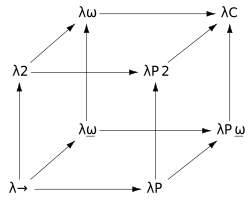
\includegraphics[scale=0.5]{lambda_cube}
\end{figure}

It covered all $8$ possibilities as analyzed above. In this paper, we will not
take an exhaustive look at all the type systems corresponding to all $8$
vertices of this cube, but highlight some prominent type systems that have been
invented.

\section{Type Theory Development}\label{sec:history}


\subsection{System F}

\emph{System F} is a Typed Lambda Calculus system that is the \emph{Simply Typed
  Lambda Calculus} but extended with \textbf{polymorphism}, meaning terms such as functions
can be created from types. A classical example is the polymorphic identity
function, which first accepts on the type of the argument given:

\[\Lambda \alpha:*.\lambda x:\alpha.x\ :\forall \alpha.\alpha \to \alpha\]

The typing rules are not described here for simplicity. An interesting result is
the Girard-Reyolds Isomorphism, named after the two researchers who
independently discovered System F, where Girard proved the Representation
Theorem and Reynolds, the Abstraction Theorem. These two theorems can be seen as
the two directions of the isomorphism between \emph{second-order polymorphic
  lambda calculus ($\lambda2$)} and \emph{second-order intuitionistic predicate logic
  (P2)}.

The idea of polymorphism is useful in programming, where a function can
``change'' its behaviour according to the type of the given input. Therefore,
System F and its extensions $F_{\omega}, F_{:>}$ which add \textbf{type operators}
and \textbf{subtyping} respectively, are often used in the implementation of
functional programming languages. For example, the Glasgow Haskell Compiler
(GHC) uses an extension of $F_{\omega}$ in its implementation.


\subsection{Calculus of Constructions}

The \textbf{Calculus of Constructions}\cite{coquand1986calculus} is a high-level
purely functional programming language, and also a type theory that is most well
known for sitting on the top of the Lambda Cube, ie., it has all the properties
of \textbf{polymorphism, type constructors and dependent types} and hence a
superset of \textbf{System F}. This system underlies the implementation of the
influential theorem prover \textbf{Coq}. The nice properties of this system
includes \textbf{strong normalization}, showing that all programs terminate, and
additionally, it is logically consistent.

There has been many extensions for \textbf{Calculus of Constructions}, one
notable example the \emph{Calculus of Inductive Constructions (CIC)}, which is
fomulated as the \textbf{Coq} theorem prover was implemented. One feature of CIC
is it improves on pure \emph{Calculus of Construction}'s drawbacks when
implemented as a theorem prover or programming language, namely that the
inductive definitions made computing functions efficiently and proving some
natural properties impossible \cite{paulin2015introduction}.


\subsection{Logical Framework}
\emph{Logical Framework (LF)} is different in its purpose from other type
theories that it is designed to be a ``general theory of logical systems that
isolates the uniformities of a wide class of logics''\cite{harper1993framework}.
It is designed to be a formal system as weak as possible, but with nice
properties that allow the representation of different type theories by
guaranteeing some normalization. On the Lambda Cube, it has the
\textbf{dependent type} feature which allows types to be created using terms.

Some central features to note about Logical Framework are on
\textbf{Definitional Equality}, which is defined between all entities (called
\emph{Kinds}, which are types of \emph{Families}, which in turn are types of
\emph{Objects}) as the transitive clousure of the \textbf{parallel nested
  reduction}, a rule based on the $\beta$-reduction in Lambda Calculus. It inherits
what is known as the Church-Rosser Property, which shows that if a Lambda
Calculus term can be reduced to two different terms, then there exist a term
where these intermediate terms can eventually converge to under reduction. As a
type system, \textbf{LF} enjoys the \textbf{strong normalizing} and
\textbf{recursively decidable} properties, making it suitable for embedding
different logics.


\subsection{Martin-Lof Type Theory}

Martin-Lof Type Theory is also known as Dependent Type Theory or Constructive
Type Theory. Invented by Martin-Lof in the 1970s, it is originally a framework
designed to rigorously formulate constructive mathematics, a branch of
mathematics that focuses on the philosophy of \emph{constructivism}, asserting
that any proof of existence of any mathematical object needs an explicit example
to be consider valid.

The logic behind this philosophy known as \emph{intuitionistic logic} or
\emph{constructive logic}, which is classical logic without the law of excluded
middle. The \emph{Law of Excluded Middle (LEM)} asserts that every proposition
is either true or false:
\[
\prftree[r]{LEM}{}{P\vee \neg P}
\]

Which leads to non-constructive existence proofs which first assume the
non-existence of the desired object, and reach a contradiction. Even though this
is sound in classical logic, it does not provide any evidence for this newly
proved existence, hence non-constructive.

Martin-Lof type theory first start off with only 3 ground types: the \emph{null
  type} \textbf{0} which has no object in the type, the \emph{unit type}
\textbf{1} which has only one object in the type, and the \emph{boolean type}
\textbf{2}, which consists of \verb|{True, False}|. All other types are
constructed via a the \emph{$\Sigma$ type} and \emph{$\Pi$ type} inductively.

Via the Curry-Howard isomorphism, the proposition claiming that two proofs $a,b$
for the same proposition $A$ are identical, $Id_{A}(a,b)$ is then a type. The
objects $p: Id_{A}(a,b)$ residing in $Id_{A}(a,b)$ are proofs that the proofs
$a,b$ are identical. An important question in mathematics was the
\textbf{Uniqueness of Identity Proof (UIP)} problem:
\begin{align*}
  \text{For any type $A$, terms $a,b:A$, can $Id_{A}(a,b)$ have more than $1$ element?}
\end{align*}

The provability of \textbf{UIP} in Martin-Lof Type Theory was the biggest open problem in
Type Theory during its time. It was finally solved by Martin Hofmann and Thomas
Streicher\cite{hofmann1998groupoid} in the negative, using an interepretation of
Types as Groupoids. This approach was later independently used by Vladimir
Voevodsky, Steve Awodey and others to create Homotopy Type Theory.

\subsection{Homotopy Type Theory}

It started with the problem in martin-lof's type theory about the identity type
and how many terms can inhabit the type. Since each term is a proof, this
translates to UIP.\@This is first proven by Hofmann and friend in 1998 or
something.

Hofmann and Streicher had a Groupoid model for intensional Martin-Lof type
theory.

In 2007, Awodey and Warren presented a novel connection between model
categories, a category with three distinguished subcategories: ``weak
equivalences'', ``fibrations'' and ``cofibrations'', which is a structure
studied in homotopy theory, a branch of algebraic topology. The explanations on
homotopy theory and category theory is out of the scope of this paper, but it is
important to recognize that the slogan of ``Proposition as Types'' from the
Curry-Howard Correspondence can be interpreted in such systems as ``Fibrations
as Types'', shedding new light to Type Theory especially in terms of identity
types. In particular, equalities are viewed as paths, dependent types are viewed
as fibrations, giving a rare geometry interpretation to the area of logic, where
diagrams are scarce.

\begin{figure}[H]
  \centering
  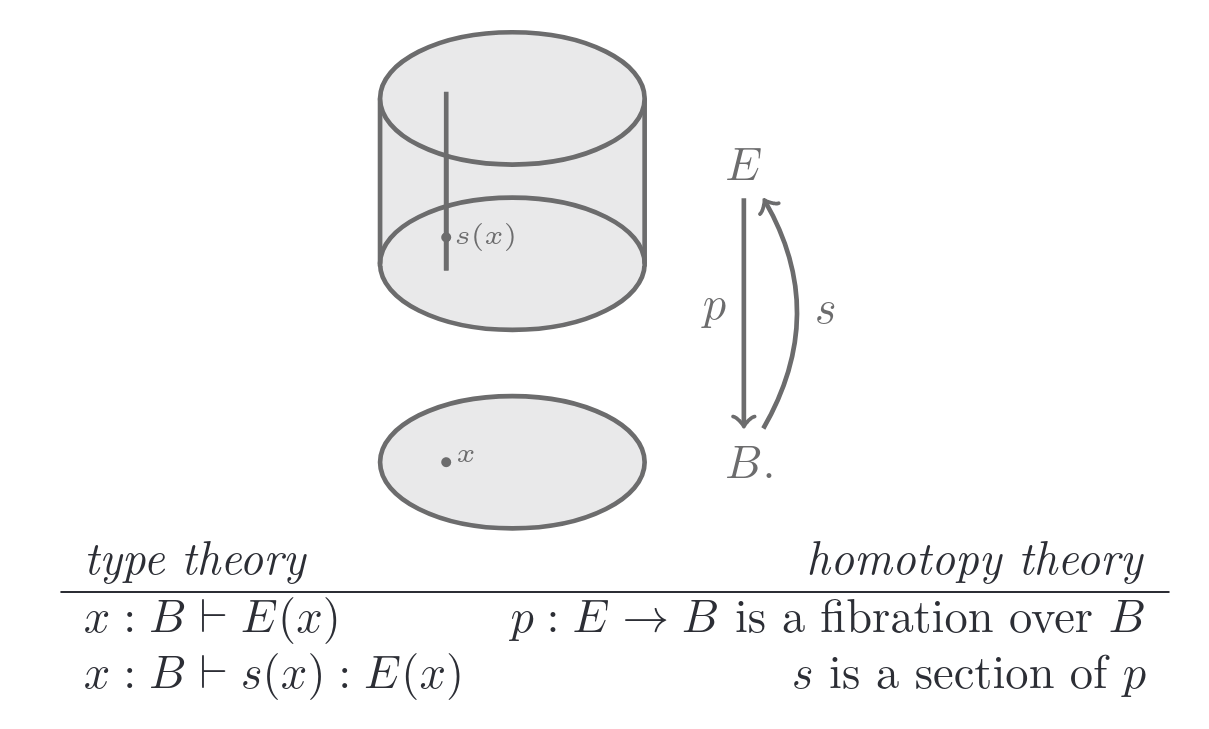
\includegraphics[scale=0.3]{fibration}
  \caption{Homotopy theoretic interpretation of dependent types
and terms (taken from~\cite{pelayo2014homotopy})}
  \Description{A cyllynder with a line across, a disc, and a commutative diagram
  expalining the fibration and section interpretation of dependent types.}
\end{figure}

In simpler terms, we have another interpretation of Type Theory through homotopy
theory in Table~\ref{tab:hott}:

\begin{table}[H]
  \caption{A simplified interpretation of Type Theory in Homotopy
    Theory\cite{awodey2013voevodskys}}
  \label{tab:hott}
\begin{tabular}{ll}
  \toprule
  Type Theory & Homotopy Theory\\
  \midrule
  Type & Space \\
  Objects & Point in space\\
  $a:A$ & $a$ is a point in the space $A$\\
  $a=b:Id_{A}(a, b)$ & $a,b$ are path connected\\
  $Id_{A}$ the type of identities & the path space of continuous maps $[0,1]\to A$\\
  $f:A\to B$ & continuous function from $A$ to $B$\\
  \bottomrule
\end{tabular}
\end{table}

The standard reference for this new innovation is the
\href{https://homotopytypetheory.org/book/}{HoTT Book}\cite{hottbook}, by the
Univalent Foundations Program of the Institute of Advanced Study.

\section{Prominent Systems using Type Theory}\label{sec:application}

\begin{table}[H]
  \caption{Systems and their Type Theory}\label{tab:systems}
  \begin{tabular}{lll}
    \toprule
    Type Theory& Systems\\
    \midrule
    System F & ML family (OCaml, Standard ML), Haskell \\
    Logical Framework & Edinburgh Logical Framework (LF), Isabelle, Twelf \\
    Calculus of Constructions & Coq, Agda \footnotemark[1]\\
    Homotopy Type Theory & Cubical Agda\cite{cohen2016cubical}\\
    Dependent Type Theory & F*, Lean, Idris, Isabelle, Agda etc. \\
    \bottomrule
\end{tabular}
\end{table}

\footnotetext[1]{Agda uses the Unified Theory of Types, which is a
  combination of Calculus of Constructions and Martin-Lof's Type Theory.}
\section{Future research directions}\label{sec:future}

As Homotopy Type Theory is the most recent system, there are many open problems,
mostly hidden behind the mathematical requirement to understand them. The
Homotopy Type Theory Summer School 2019 (HoTT2019) has collated a list of open
problems from the speakers, and the nLab website, an initiative to promote the
use of Category Theory, has a good collection of open problems on HoTT as well
(\cite{hottOpenProblem}, \cite{hottOpenProblem2019}).


\bibliographystyle{ACM-Reference-Format}
\bibliography{references}
% \appendix
% \section{Definition of common terminologies in Type Theory}
% \begin{itemize}
% \item \textbf{Propositional Logic}: also known as \textbf{Zeroth-order Logic},
%         is the logical system with only the connectives $\wedge, \vee, \neg, \implies$ and
%         no free variables.
% \item \textbf{Predicate Logic}: also known as \textbf{First-order Logic}, is the
%         logical system with quantifiers.
% \end{itemize}
\end{document}
